\documentclass{standalone}
\usepackage{tikz}

\begin{document}

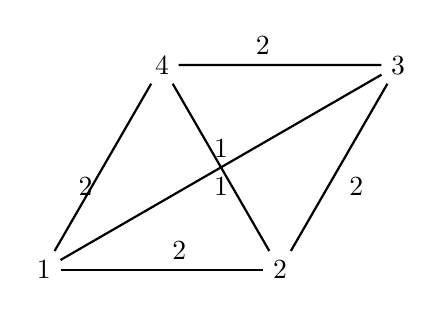
\begin{tikzpicture}[scale=1.5]
    % Define the vertices
    \node (v1) at (0,0) {1};
    \node (v2) at (2,0) {2};
    \node (v3) at (3,1.732) {3};
    \node (v4) at (1,1.732) {4};

    % Draw the edges
    \draw[thick] (v1) -- node[midway, above right] {2} (v2);
    \draw[thick] (v2) -- node[midway, below right] {2} (v3);
    \draw[thick] (v3) -- node[midway, above left] {2} (v4);
    \draw[thick] (v4) -- node[midway, below left] {2} (v1);

    % Draw additional edges for the ring structure
    \draw[thick] (v1) -- node[midway, above] {1} (v3);
    \draw[thick] (v2) -- node[midway, below] {1} (v4);
\end{tikzpicture}

\end{document}